\chapter*{Appendix}

\section*{Hazelcast on EC2 Tutorial}
This is a step by step tutorial how to configure a very basic Hazelcast cluster inside Amazon EC2. This tutorial excepts that you have ssh available (on windows you can use Putty) and that you have an Amazon EC2 account. You also need to have the Amazon access key and secret key. The access key should look like this: 

BNELSKS9B8LDLE8NXKKA 

and your secret key should look like this:

384c32KDLLDM44l3l3lddudueIEEL/Uldlx395uM

First we login to the management console, e.g. 

https://console.aws.amazon.com/ec2/v2/home?region=eu-west-1. 

There we press the "Launch Instance" button.

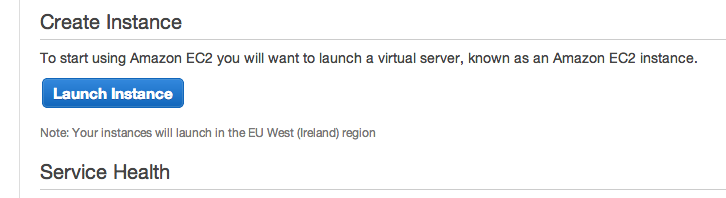
\includegraphics[scale=0.30]{ec2-0.png}

Select 'classic wizzard'.

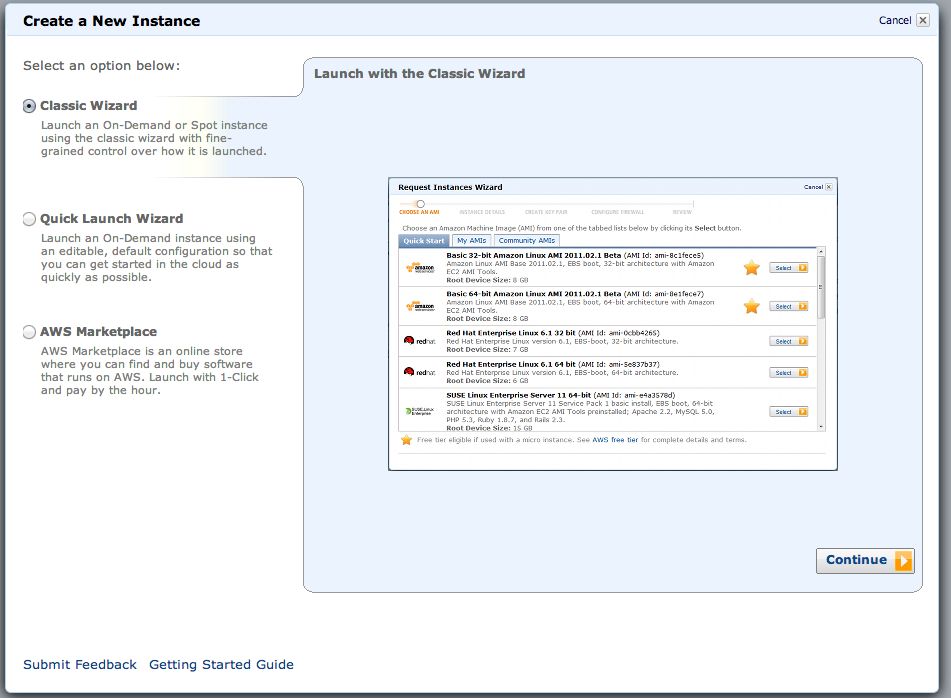
\includegraphics[scale=0.30]{ec2-1.png}

Select 'Ubuntu Server 12.10'

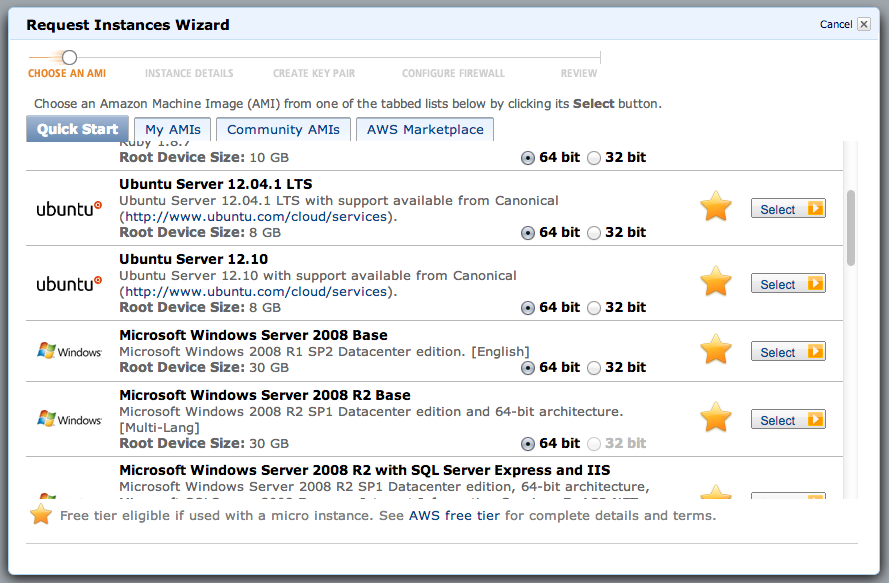
\includegraphics[scale=0.30]{ec2-2.png}

We are going to create 2 ubuntu servers at once. So enter 2 for "Number of instances" and press continue.

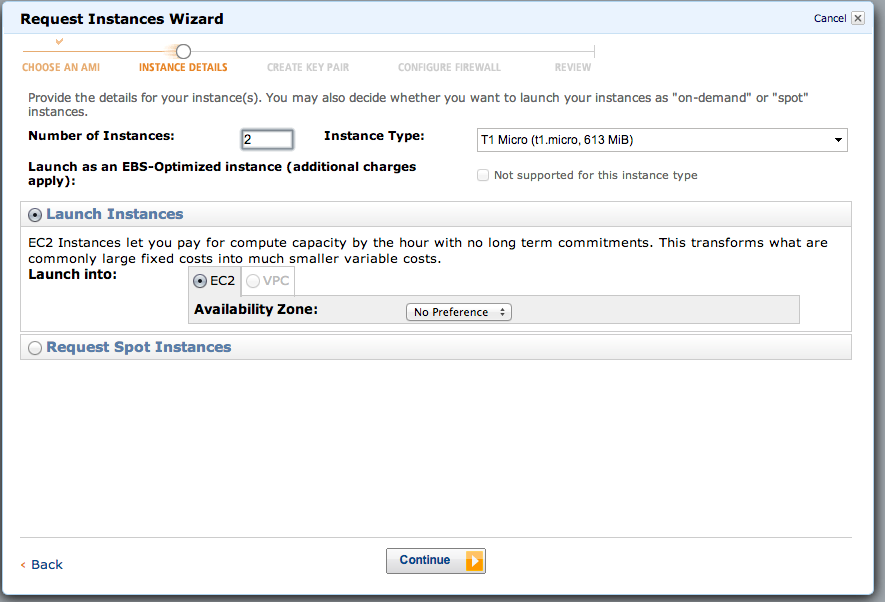
\includegraphics[scale=0.30]{ec2-3.png}

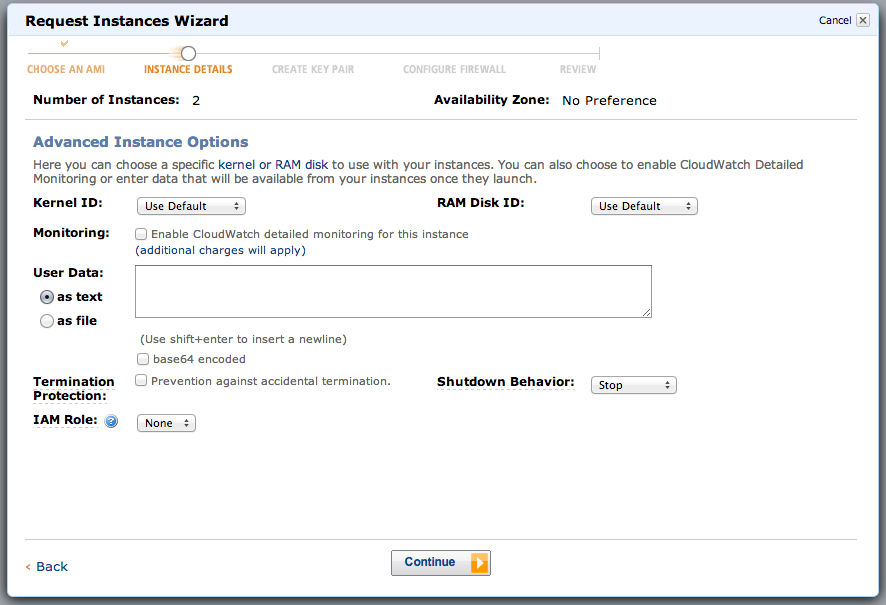
\includegraphics[scale=0.30]{ec2-4.png}

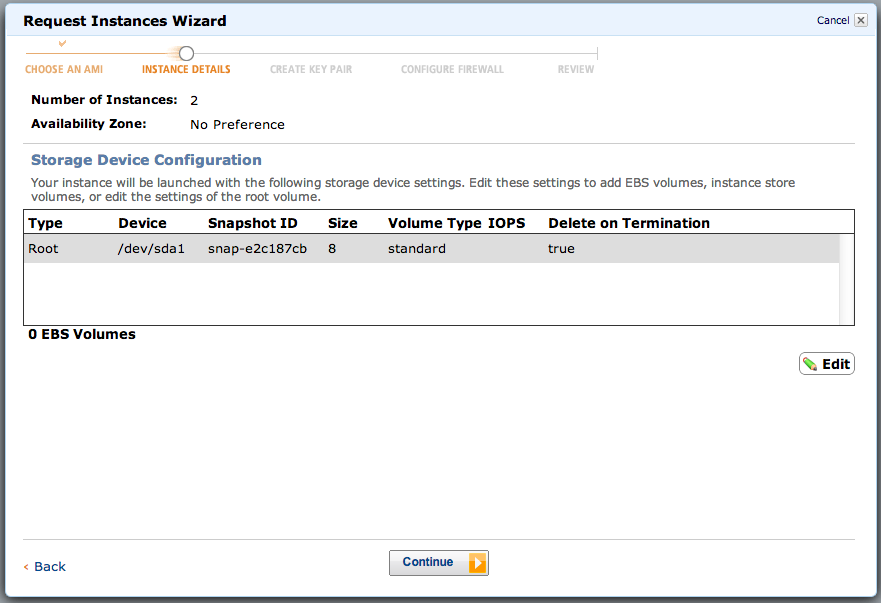
\includegraphics[scale=0.30]{ec2-5.png}

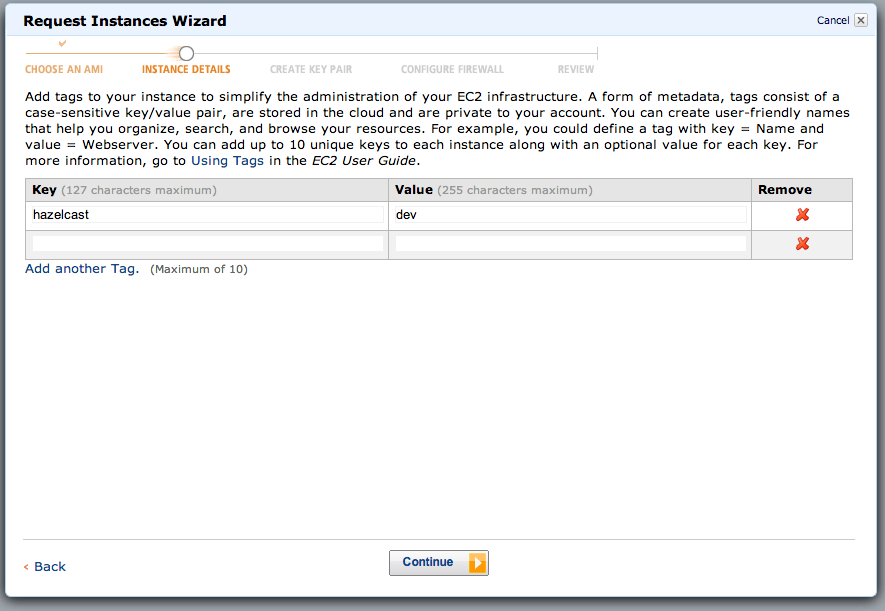
\includegraphics[scale=0.30]{ec2-6.png}

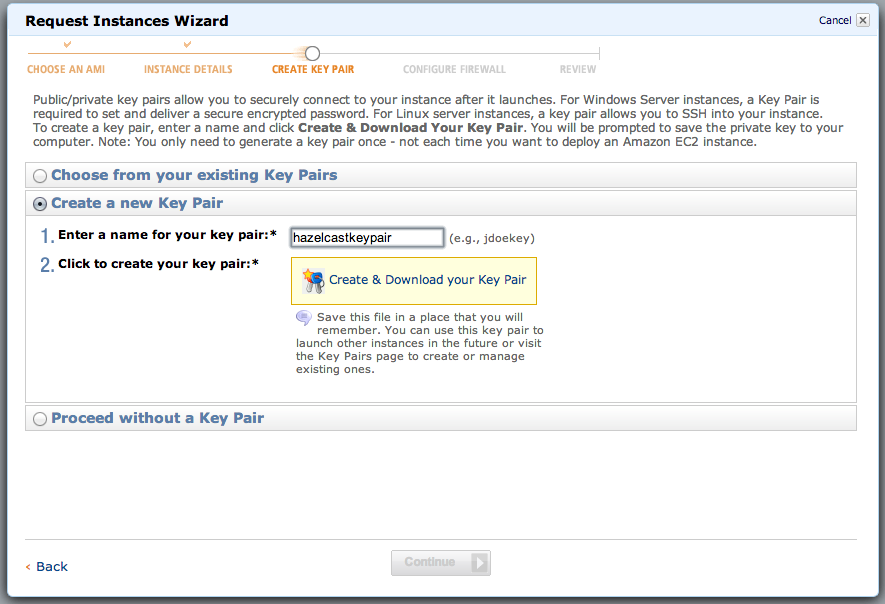
\includegraphics[scale=0.30]{ec2-7.png}

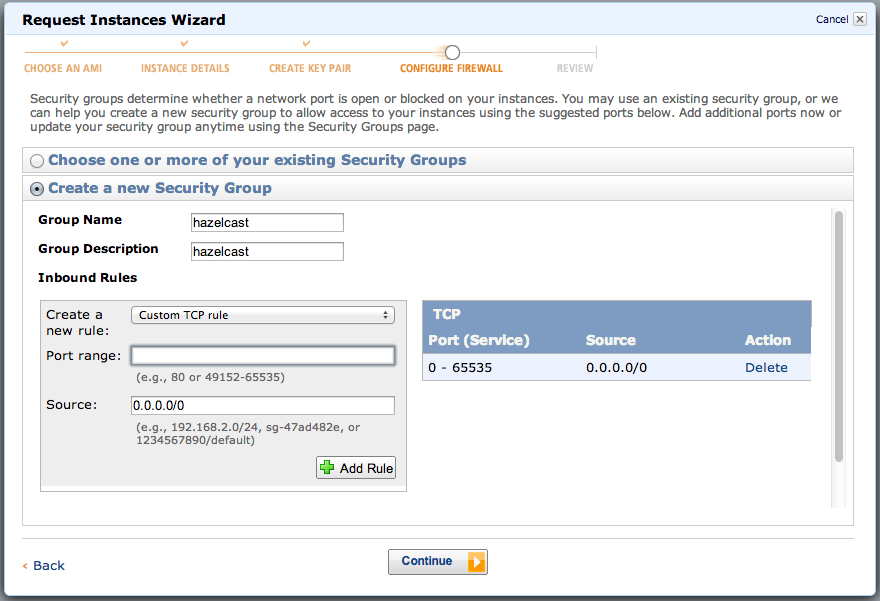
\includegraphics[scale=0.30]{ec2-8.png}

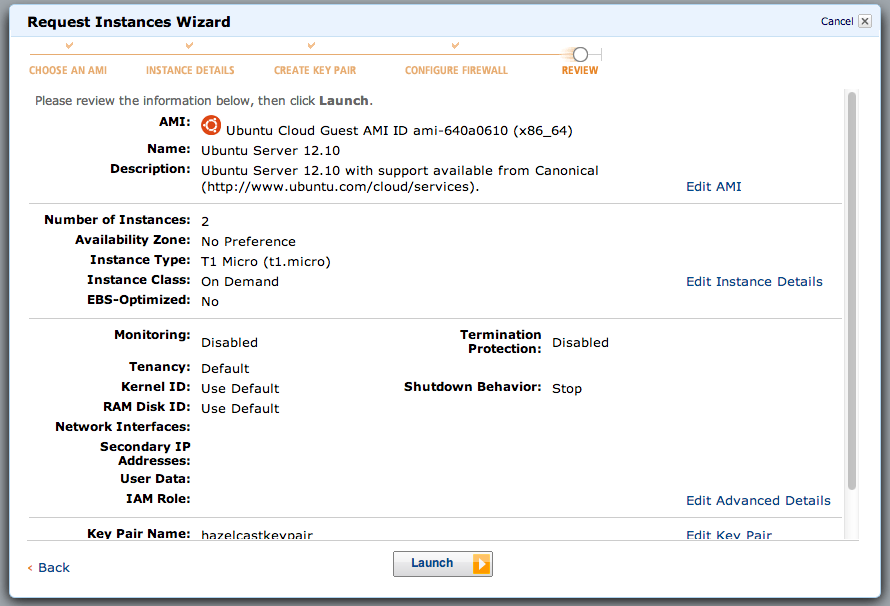
\includegraphics[scale=0.30]{ec2-9.png}

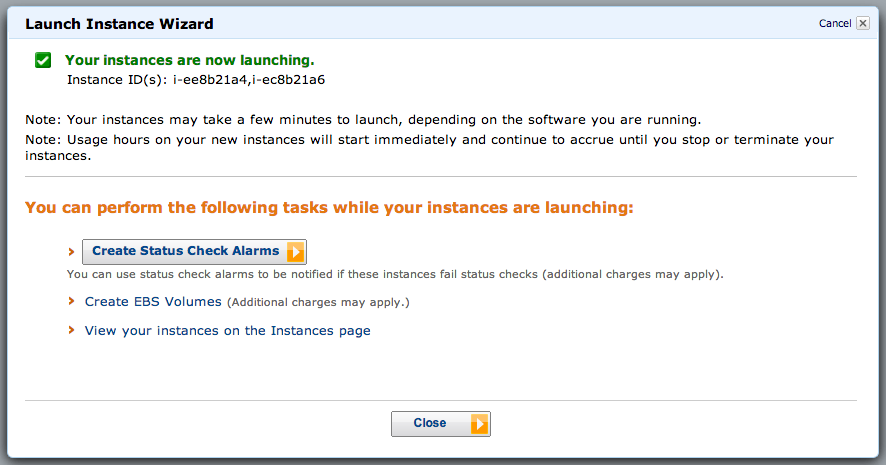
\includegraphics[scale=0.30]{ec2-10.png}